\begin{gather*}
    V_1 = 1 + (5 + 6) \mathrm{mod} 5
    = 1 + 11 \mathrm{mod} 5
    = 1 + 1 = 2\\
    V_2 = 6 + (5 + 6) \mathrm{mod} 5
    = 6 + 11 \mathrm{mod} 5
    = 6 + 1 = 7\\
\end{gather*}

\subsection{Вариант 2}
Топология:
\begin{center}
    \begin{tikzpicture}
        \node[draw,circle] (1) at (-4, 3) {1};
        \node[draw,circle] (2) at (-4, -3) {2};
        \node[draw,circle] (3) at (0, 0) {3};
        \node[draw,circle] (4) at (5, 0) {4};
        \draw (1) -- (2);
        \draw (1) -- (3);
        \draw (2) -- (3);
        \draw (3) -- (4);

        \draw[-stealth, thick, transform canvas={yshift=-0.5em}] (4) -- (3);
        \draw[-stealth, thick, transform canvas={xshift=0.3em,yshift=-0.4em}] (3) -- (2);
        \draw[-stealth, thick, transform canvas={xshift=-0.5em}] (2) -- (1);

        \draw[-stealth, thick, dotted, transform canvas={xshift=-1em}] (1) -- (2);
        \draw[-stealth, thick, dotted, transform canvas={xshift=0.6em,yshift=-0.8em}] (2) -- (3);
        \draw[-stealth, thick, dotted, transform canvas={yshift=-1em}] (3) -- (4);
    \end{tikzpicture}
\end{center}

На компьютерах должна быть настроена маршрутизация таким образом,
чтобы запросы от \texttt{nc client 1} к \texttt{nc server} проходили через компьютер 2,
запросы от \texttt{nc client 2} к \texttt{nc server} проходили через компьютер 1.

Сплошными стрелками на рисунке обозначен путь запроса от \texttt{nc client 1} к \texttt{nc server},
штриховыми --- путь ответа от \texttt{nc server}.

\subsection{Вариант 7}

\begin{center}
    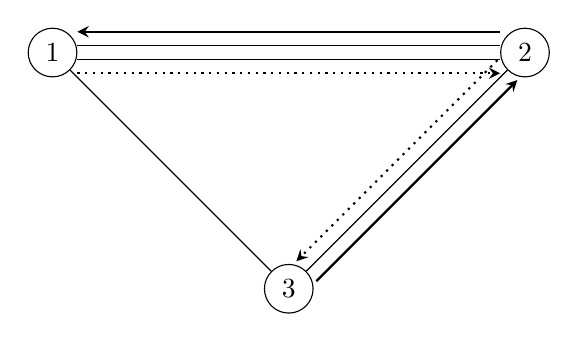
\begin{tikzpicture}
        \node[draw,circle] (1) at (0, 0) {1};
        \node[draw,circle] (2) at (6, 0) {2};
        \node[draw,circle] (3) at (3, -3) {3};

        \draw[transform canvas={yshift=0.25em}] (1) -- (2);
        \draw[transform canvas={yshift=-0.25em}] (1) -- (2);
        \draw (1) -- (3);
        \draw (2) -- (3);

        \draw[-stealth, thick, transform canvas={yshift=0.75em}] (2) -- (1);
        \draw[-stealth, thick, transform canvas={xshift=0.36em,yshift=-0.36em}] (3) -- (2);
        \draw[-stealth, thick, dotted, transform canvas={yshift=-0.75em}] (1) -- (2);
        \draw[-stealth, thick, dotted, transform canvas={xshift=-0.36em,yshift=0.36em}] (2) -- (3);
    \end{tikzpicture}
\end{center}

Между компьютерами 1 и 2 проведено 2 изолированных друг от друга канала.
IP1 --- адрес интерфейса в компьютере 1, подключенный к каналу 1.
IP2 --- адрес интерфейса в компьютере 2, подключенный к каналу 1.

Необходимо настроить таблицы маршрутизации и правила выбора таблиц маршрутизации таким образом,
чтобы ICMP Echo Request, отправленный с компьютера 3 на IP1,
прошел через компьютер 2 и канал 1 (сплошные стрелки на рисунке),
а ICMP Echo Reply прошел через канал 2 в компьютер 2, после чего отправился в компьютер 3.
ICMP Echo Request, отправленный с компьютера 3 на IP2 прошел через компьютер 1 и канал 1,
а ICMP Echo Reply прошел через канал 2 в компьютер 1, после чего отправился в компьютер 3.

В отчете в дополнение к общим пунктам нужно предоставить доказательства того,
что каналы 1 и 2 изолированы друг от друга (например,
в виде скриншотов дампов трафика и распечатки логов тестирования).
